


\documentclass{article}[12pt]
\usepackage{fullpage,graphicx, setspace, latexsym, cite,amsmath,amssymb,color,subfigure}
%\usepackage{epstopdf}
%\DeclareGraphicsExtensions{.pdf,.eps,.png,.jpg,.mps} 
\usepackage{amssymb} %maths
\usepackage{amsmath} %maths
\usepackage{amsthm}

\bibliographystyle{unsrt}

\newtheorem{theorem}{Theorem}
\newtheorem{prop}{Proposition}
\newtheorem{corollary}{Corollary}
\newtheorem{lemma}{Lemma}
\newtheorem{defn}{Definition}
\newtheorem{ex}{Example}
\usepackage{float}

\def\R{\mathbb{R}}
\def\Eps{\mathcal{E}}
\def\E{\mathbb{E}}
\def\V{\mathbb{V}}
\def\F{\mathcal{F}}
\def\G{\mathcal{G}}
\def\H{\mathcal{H}}
\def\S{\mathcal{S}}
\def\P{\mathbb{P}}
\def\1{\mathbf{1}}
\def\n{\nappa}
\def\h{\mathbf{w}}
\def\v{\mathbf{v}}
\def\x{\mathbf{x}}
\def\X{\mathcal{X}}
\def\Y{\mathcal{Y}}
\def\eps{\epsilon}
\def\y{\mathbf{y}}
\def\e{\mathbf{e}}
\newcommand{\norm}[1]{\left|\left|#1\right|\right|}
\DeclareMathOperator*{\argmin}{arg\,min}
\DeclareMathOperator*{\argmax}{arg\,max}

\newcommand{\lecture}[4]{
   \pagestyle{myheadings}
   \thispagestyle{plain}
   \newpage
   % \setcounter{lecnum}{#1}
   \setcounter{page}{1}
   \setlength{\headsep}{10mm}
   \noindent
   \begin{center}
   \framebox{
      \vbox{\vspace{2mm}
    \hbox to 6.28in { {\bf ESE 680-004: Learning and Control
   \hfill Fall 2019} }
       \vspace{4mm}
       \hbox to 6.28in { {\Large \hfill Lecture #1: #2  \hfill} }
       \vspace{2mm}
       \hbox to 6.28in { {\it Lecturer: #3 \hfill Scribes: #4} }
      \vspace{2mm}}
   }
   \end{center}
   \markboth{Lecture #1: #2}{Lecture #1: #2}

   \noindent{\bf Disclaimer}: {\it These notes have not been subjected to the
   usual scrutiny reserved for formal publications. }
   \vspace*{4mm}
}

%notation

\def \E{\mathbb E}
\def \P{\mathbb P}
\def \R{\mathbb R}
\def \A{\cal A}

\begin{document}

\lecture{15}{Most of Statistical Learning theory}{Nikolai Matni}{Shuo Li}

\section{A Simple Problem}
\
\indent Before diving into statistical learning theory, we first setup a problem our learner might be faced with. The book used papaya example to illustrate its idea, while we would use a robotics example. Since analysis in the book mainly focuses on binary classification problem, we would also start from a binary classification problem in robotics.

Suppose that we want to train a learner to detect anomaly of an vehicle engine. We have features like engine's sound, weight, temperature and outside weather. After doing some experiments, we collected some training data of different engine states with corresponding features. The goal is to get a model which could accurately detect anomaly basing on such features using training data we have.

In the example above, the statistical learning theory aims to formally measure how well our model could perform on data we have not seen before, or generalize to testing data.

\section{The Statistical Learning Framework}
In this part, we set up a formal model on which we build our analysis.

\begin{enumerate}
    \item \textbf{The model's input:}
    \begin{enumerate}
        \item \textbf{Domain set:} An arbitrary set, $\mathcal{X}$. This is the set of objects that we may wish to label. For instance, in the engine anomaly detection case, the domain set is all combinations of different features, including sound, weight, temperature and weather. These features could be real values or logical integers.
        \item \textbf{Label Set}: The set of possible labels, $\mathcal{Y}$. For our current discussion, we will restrict the label set to be a two-element set, i.e.$\{-1,1\}$ or $\{0, 1\}$. In our case, we define our label set as $\{0,1\}$ where 0 means normal state, 1 means anomaly.
        
        In other problems, including multi-classification or regression, the label set could also be sets of logical integers or real values.
        \item \textbf{Training Set:} $S=\{(x_1,y_1)\ldots,(x_m,y_m)\}$ is a finite sequence of pairs in $\mathcal{X}\times\mathcal{Y}$: that is, a sequence of labeled domain points. In our engine case, the training set is the (features, engine states) training dataset we collected through experiments.
    \end{enumerate}
    \item \textbf{The Model's Output:} The learner is requested to output a prediction rule, $f: \mathcal{X} \rightarrow \mathcal{Y}$. This function is also called a predictor, a hypothesis, or a classifier (or regressor in regression problems). The predictor can be used to predict the label of new domain points. In our case, the predictor is the one trained upon training set. We are going to use this model to detect anomaly. We use $A(S)$ to denote the hypothesis (predictor) that a learning algorithm, A, returns upon receiving the training sequence S.
    \item \textbf{The Generative Model in Nature:} We assume that the instances are generated by some probability distribution. Using Bayesian Rule, we can write the generative probability as $p(x,y)=p(x)*p(y|x)$, where $x \in \mathcal{R}^4$ is the feature vector, $y$ is the engine state. Let us denote that probability over $\mathcal{X}$ by $\mathcal{D}$. It is important to note that we do not assume that the learner knows anything about this distribution. Actually, our predictor is expected to learn this probability through training data. We denote the generative model as $g: \mathcal{X} \rightarrow \mathcal{Y}$, and that $y_i=f(x_i)$ for all i. In our engine case, $g$ is the function that project our input features onto different engine states.
    
    \item \textbf{Measures of success:} We define the error of a classifier (predictor) to be the probability that it does not predict the correct label on a random data point generated by the aforementioned underlying distribution. In our engine case, the measure of success is the probability that the prediction is correct basing on input features using the trained predictor.
    
    Formally, given a domain subset, $A \subset \mathcal{X}$, the probability distribution $\mathbb{D}$, assigns a number, $\mathcal{D}(A)$, which determines how likely it is to observe a point. In many cases, we refer to A as an event and express it using a function $\pi: \mathcal{X} \rightarrow \{0,1\}$, namely, $A=\{x \in \mathcal{X}: \pi(x)=1\}$. In that case, we also use the notation $\mathbb{P}_{\x \thicksim \mathcal{D}}[\pi(x)]$ to express $\mathcal{D}(A)$.
    
    We define the error of a prediction rule: $h: \mathcal{X} \rightarrow \mathcal{Y}$, to be
    \begin{equation}
        Loss_{\mathcal{D}}(f(x),y) \equiv \mathbb{P}_{x \thicksim \mathcal{D}}[h(x)\neq f(x)] \equiv \mathcal{D}(\{x: f(x)\neq y\})
    \end{equation}
    That is, the error of such $h$ is the probability of randomly choosing an example x for which $h(x)\neq f(x)$. The subscript $(\mathcal{D},f)$ indicates that the error is measured with respect to the probability distribution $\mathcal{D}$ and the correct labeling function $f$.
    \item \textbf{A Note About the Information Available to the Learner:} The learner is blind to the underlying distribution $\mathcal{D}$ over the world and to the labeling function $f$. In our engine example, we have no knowledge about how to bind engine states with its sound, weight, temperate and outside weather. The only way the learner can interact with the environment is through collected training dataset.
\end{enumerate}

\section{Empirical Risk Minimization}
As mentioned earlier, a learning algorithm receives as input a training set S, sampled from an unknown distribution $\mathcal{D}$ and labeled by some target function $g$, and should output a predictor $f_S: \mathcal{X} \rightarrow \mathcal{Y}$. The goal of the predictor is to find $f_S$ that could achieve the lowest prediction error with respect to the unknown $\mathcal{D}$ and $g$.

However, since the learner does not know what $\mathcal{D}$ and $g$ are, the \textbf{empirical error} or \textbf{empirical risk} which could be calculated by the learner is often used as the proxy of the true error. The error on training error is as 
\begin{equation}
    Loss_{S} (f_S(x),y)\equiv \frac{|\{i \in [m]: f_S(x_i)\neq y_i\}|}{m}
\end{equation}where $[m]=\{1,\ldots,m\}$.

Since the training dataset is the snapshot of the world that is available to the learner, it makes sense to search for a solution that works well on that data. The learning paradigm - coming up with a predictor h that minimizes $L_S(f_S(x),y)$ - is called \textit{Empirical Risk Minimization} or ERM for short.

Note that, in classification case, the empirical risk is the error rate on the training dataset. In regression problems, the empirical risks could be formalized as the Mean Squared Error loss on training dataset, i.e.
\begin{equation*}
    L_S (f_S(x),y)= \frac{1}{m} \sum_{i=1}^m \|f_S(x_i)-y_i\|^2
\end{equation*}

\section{True Risk V.S. Empirical Risk: Overfitting}
\
\indent Although the empirical risk minimization algorithm seems reasonable, the fact that the training dataset might be non representative of the true distribution may cause the predictor learned upon the training dataset to overfit. That is, the predictor might perform well or perfectly (i.e. achieve zero empirical loss on training dataset), but poorly on the true distribution. 

For instance, consider the following predictor:
\begin{equation*}
f_S(x) = 
\left\{ \begin{array}{rl}
y_i & \mbox{if} \ \exists i \in [m] \ s.t. \ x_i=x \\
0 & \mbox{otherwise}
\end{array}\right.    
\end{equation*}
Clearly, no matter what the sample is, $L_S(h_S)=0$, and therefore this predictor may be chosen by an ERM algorithm (it is one of the empirical-minimum-cost predictor; no predictor can have smaller error). On the other hand, since the predictor almost always predict 0 for any x, the true error rate of this predictor is approximately 1/2. Thus, $L_{\mathcal{D}}=1/2$. We have found a predictor whose performance on the training dataset is excellent yet its performance on the true distribution is very poor (as poor as random predictor). This phenomenon is called \textit{overfitting}.

Formally, we could also decouple the true risk as follows:
\begin{equation*}
    L_{\mathcal{D}}(f_S(x),y) = L_{\mathcal{D}}(f_S(x),y) - L_{\mathcal{S}}(f_S(x),y)  + L_{\mathcal{S}}(f_S(x),y) 
\end{equation*}
We define the term $L_{\mathcal{D}}(f_S(x),y)  - L_{\mathcal{S}}(f_S(x),y) $ as \textit{generalization risk}, while the second term is actually \textit{empirical risk}.

\section{The Independently and Identically Distributed (i.i.d) Assumption}
Clearly, any guarantee on the error with respect to the underlying true distribution, $\mathcal{D}$, for an algorithm that has access only to a sample S should depend on the relationship between $\mathcal{D}$ and S. The common assumption in statistical machine learning is that the training sample S is generated by sampling points from the distribution $\mathcal{D}$ independently of each other. Formally, we define i.i.d assumption as

\begin{itemize}

    \item \textbf{The i.i.d assumption:} The examples in the training set are independently and identically distributed according to the distribution $\mathcal{D}$. That is, every $x_i$ in S is freshly sampled according to $\mathcal{D}$ and then labeled according to the generative function, $f$. We denote this assumption by $S \thicksim \mathcal{D}^m$ where m is the size of S, and $\mathcal{D}^m$ denotes the probability over m-tuples induced by applying $\mathcal{D}$ to pick each element of the tuple independently of the other members of the tuple.
\end{itemize}

By using the i.i.d assumption, we could get that 
\begin{equation*}
    \mathbb{E}[L_S(f_S(x),y)]= L_{\mathcal{D}}(f_S(x),y) 
\end{equation*}In other words, the expectation of empirical loss equals to the true loss. As a result, concentration bounds may help to compute the bound on generalization risk.

Actually, because of the i.i.d assumption, we can say \textbf{Learning theories tries to formalize the intuition \textit{if there's enough data, this (empirical risk) should approximate the true risk.}}


\section{Hoeffding's Inequality and McDiarmid's Inequality}

\subsection{Hoeffding's Inequality}

Hoeffding’s inequality is a powerful technique—perhaps the most important
inequality in learning theory—for bounding the probability that sums of
bounded random variables are too large or too small.

\textbf{Hoeffding's Inequality:}For a random variable X, with $\mathbb{E}(X)=0$ and $a\leq X\leq b$,then for $s > 0$
\begin{equation*}
    \mathbb{E}(e^{sX}) \leq e^{s^2(b-a)^2}/8
\end{equation*}

\subsection{McDiarmid's Inequality\cite{mcdiarmid_1989}}
Let$Z_1,\ldots, Z_n$ be independent random variables taking values in $\mathcal{Z}$. Suppose that $F: \mathcal{Z}^n \rightarrow \mathbb{R}$ satisfies
\begin{equation*}
    \sup_{(z_1,\ldots,z_n),\hat z_i} |F(z_1, \ldots, z_n)-F(z_1,\ldots,z_{i-1},\hat z_i, z_{i+1},\ldots,z_n)| \leq c_i
\end{equation*}
Then, 
\begin{equation}
    \mathbb{P}[F(Z_1,\ldots,Z_n)-\mathbb{E}[F]\geq t] \leq \exp{(-\frac{2t^2}{\sum_{i=1}^n c_i^2})}
\end{equation}


Hoeffding’s Inequality is a special case of McDiarmid’s Inequality. We require that the
random variables $Z_1, . . . , Z_n$ are i.i.d, and $Z_i \in [0,1]$. Then, we define $f(Z_1, \ldots , Z_n) = \frac{1}{m}\sum_{i=1}^n Z_i$. Note that because the $Z_i$’s are constrained to be either 0 or 1, changing one of these values will change the value of $f(Z_1, \ldots, Z_n)$ by at most $\frac{1}{m}$. So, we set $c_i =\frac{1}{m}$ in
McDiarmid’s Inequality to get the required result.

% \textbf{Reference and proof}

\section{Generalization Bound}
\
\indent In this section, we want to get the upper bound of generalization. Specifically, given a distribution $\mathcal{X}$, a finite collection of possible prediction functions $\mathcal{F}$, and a sample set sampled from $\mathcal{X}$, we want to get the upper true loss bound of a given predictor $f \in \mathcal{F}$ over distribution $\mathcal{X}$, which we denote as $R[f]$.

\subsection{Post-hoc Validation}
\
\indent Our idea is to get the generalization bound using McDiarmid's inequality. Firstly, we assume that losses are bounded, i.e. given a function (predictor) $f \in \mathcal{F}$,
\begin{equation*}
    |Loss_{\mathcal{S}}(f_S(x),y)| \leq B \  \text{for all} (x,y) 
\end{equation*}
Then, we define variable $Z_i = Loss_S(f_S(X_i),Y_i)$, and rewrite empirical loss as 
\begin{equation*}
    F(z_1,\ldots,z_n) = -\frac{1}{n}\sum_{i=1}^n Loss_S(f_S(x_i),y_i) = -R_S{[f]}
\end{equation*}Note that, true loss equals to the expectation of empirical loss, i.e.
\begin{equation*}
    \mathbb{E}[R_S(f)] = R[f]
\end{equation*}
Also, because the loss is bounded, we could use McDiarmid's Inequality to get the upper bound of generalization, i.e. let $c_i \equiv 2B/n$, $t = \epsilon$, we could get 
\begin{equation}
    \mathbb{P}[R[f]-R_S[f]\geq \epsilon] \leq \exp{(-\frac{n\epsilon^2}{2B^2})}
    \label{generalization bound}
\end{equation}By inverting \ref{generalization bound}, we could get that with probability at least $1-\delta$ we have 
\begin{equation}
    R[f] \leq R_S[F] + B\sqrt{\frac{2\log(1/\delta)}{n}}
\end{equation}

\subsection{Uniform Convergence}
\
\indent By far, we are able to get the generalization bound for a given function (predictor) $f \in \mathcal{F}$. In general, we want to evaluate the generalization bound of an algorithm $\mathcal{A}$ over a sample set S. In this case, the variables $Z_i=loss(f_S(X_i),Y_i)$ are no longer independent (\textbf{because predictors would use the same samples}), which does not satisfy the assumption of McDiarmid's Inequality.

Therefore, instead of evaluating a specific function $f_S$ output by algorithm $\mathcal{A}$, i.e. $A(S)=f_S$, we instead want to proof that the  generalization upper bound over the entire hypothesis space is small, i.e. we want to bound 
\begin{equation*}
    \mathbb{P}[\sup_{f \in \mathcal{F}}(R[f]-R_S[f]) \geq \epsilon]
\end{equation*}
or equivalently,
\begin{equation*}
    \mathbb{P}[\exists f \in \mathcal{F} : R[f] - R_S[f] \geq \epsilon] 
\end{equation*}

\subsubsection{Finite Function Class}
\
\indent We first consider the uniform convergence for finite function class. Suppose $\mathcal{F}$ is a finite collection of possible prediction functions, and assume that for all $f \in \mathcal{F}$, $x \in \mathcal{X}$, and $y \in Y$, $|\ell(f(x),y)| \leq B$. Using Ineq. \ref{generalization bound}, we could get that for a given function $f$, 
\begin{equation*}
    \mathbb{P}[R[f]-R_S[f]\geq \epsilon] \leq \exp{(-\frac{n\epsilon^2}{2B^2})} 
\end{equation*}By union bound, we could extend above inequality to the whole function space, i.e.
\begin{align}
    \mathbb{P}[\exists f \mathcal{F} : R[f]-R_S[f] \geq \epsilon] &\leq |\mathcal{F}| \mathbb{P}[R[f]-R_S[f]\epsilon]\\ &\leq |\mathcal{F}| \exp{(-\frac{n\epsilon^2}{2B^2})} 
\end{align}where $|\mathcal{F}|$ is the number of possible functions. By inverting above inequality, we could get 
\begin{equation*}
    R[f] \leq R_S[f] + B\sqrt{\frac{2\log(|\mathcal{F}/\delta|)}{2n}} \ \forall f \in \mathcal{F}
\end{equation*}

\subsubsection{Infinite Function Class}
\
\indent We start from threshold functions to study the generalization bound for infinite function class. Firstly, in our example, the threshold function is defined as 
\begin{equation*}
    F := {f_a: f_a(x) = \mathbb{I}(x<a), a \in \mathbb{R}}
\end{equation*}
Obviously, $|\mathcal{F}| = \infty$, where in fact $\mathcal{F}$ is uncountably infinite. Now consider a random variable $x \sim p(x)$, and assume that $X \in (-\infty, a_*\}$, for some unknown $a_*$. Define the loss function to be
$$
loss_S(f_a(x),x) = 1-f_a(x)=\left\{ \begin{array}{rcl}
0 
& \text{if} \ x < a \\ 1 & \text{otherwise}
\end{array}\right.
$$

Then, $R[f_a]=\mathbb{E}_x[1-f_a(x)] = \mathbb{P}[x \in [a, a_*]]$, and $R[f_{a_*}]=0$. The empirical risk is given by $R_S[f_a] = \frac{1}{n}\sum_{i=1}^n 1-f_a(x_i)$. We then sample $S=(x_1, \ldots, x_n)$ and set $\hat a=max_i x_i$. Note that by construction, $\hat a$ is an empirical risk minimizer achieving $R_S[f_{\hat a}]=0$.

We want to bound $\mathbb{P}[R[f_{\hat a}]-R_S[f_{\hat a}]\geq \epsilon] = \mathbb{P}[R[f_{\hat a}\geq \epsilon]|R_S[f_{\hat a}]=0]$, i.e. probability of drawing $S=(x_1, \ldots, x_n)$ s.t. $R_S[f_{\hat a}]=0$ but $R[f_{\hat a}]$ is large. A demonstration of the error probability is as Fig.\ref{empirical}.

\begin{figure}[H]
    \centering
    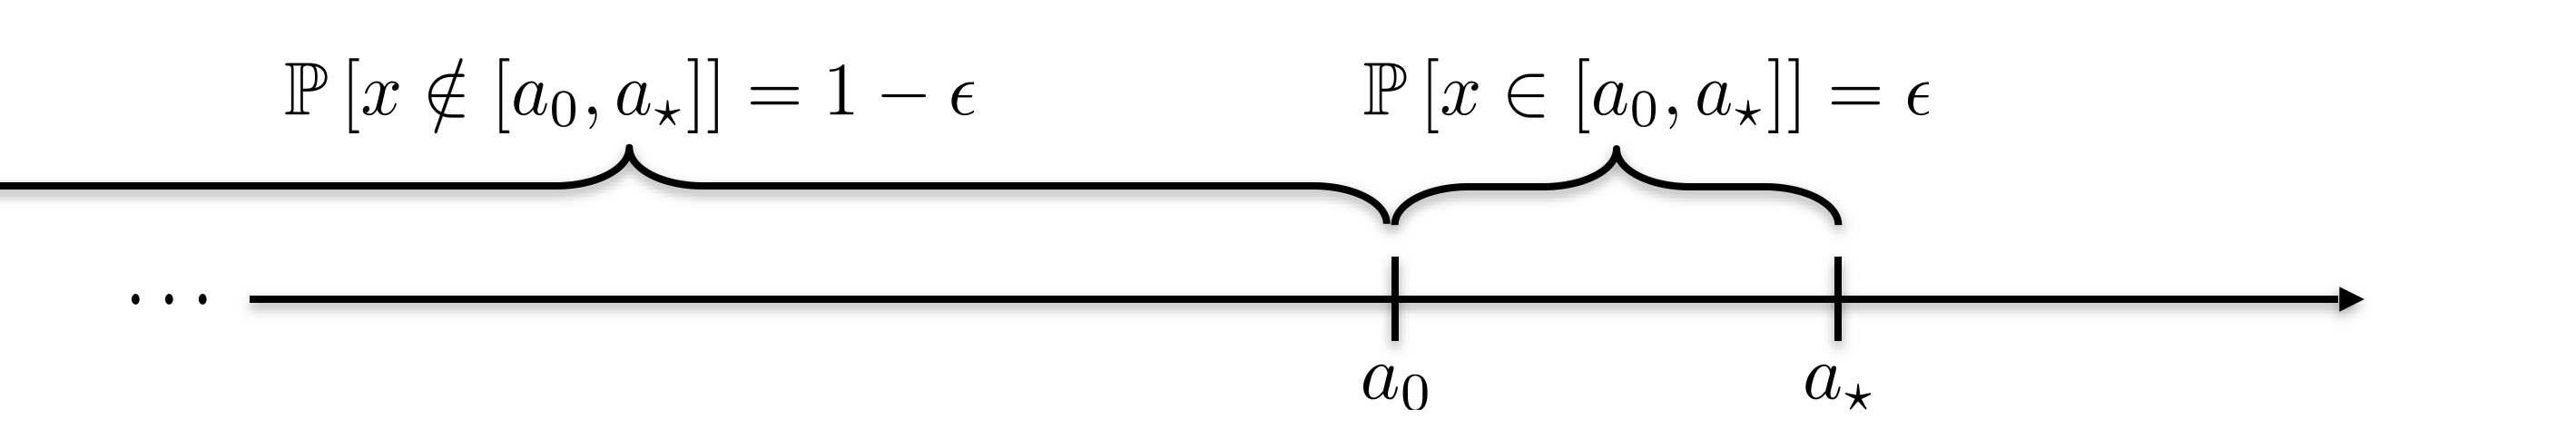
\includegraphics[scale=0.3]{figures/example.png}
    \caption{Demonstration of the error probability}
    \label{empirical}
\end{figure}

Recall that we set $\hat a = \max_i x_i$. Therefore, the only way to achieve $R_S[f_{\hat a}]=0$ and $R[f_{\hat a}] \geq \epsilon$ is if $x_i \notin [a_0, a_*]$ for all $i=1,\ldots,n$
\begin{align*}
        \mathbb{P}[R[f_{\hat a}]\geq \epsilon] &= \mathbb{P}[x_i \notin [a_0, a_*] \ \forall i=1,\ldots, n]\\
        &= (\mathbb{P}[x \notin [a_0, a_*]])^n \ \text{since} x_i \stackrel{i.i.d}{\sim} p(x)\\
        &= (1-\epsilon)^n \leq e^{-\epsilon n}
\end{align*}

By inverting above inequality, we could get that 
\begin{equation}
    R[f_{\hat a}] = \mathbb{P}[x \in [\hat a, a_*]] \leq \frac{\log(1/\delta)}{n}
\end{equation}

This example tells two things. First, it is the "expressiveness" of $\mathcal{F}$ that matters, not its cardinality. Specifically, the cardinality of threshold function is infinite, but the generalization bound is finite. Second, if the function class $\mathcal{F}$ and data satisfy a realizability assumption, i.e. $\exists f_* \in \mathcal{F}$ such that $R[f_*]=0$, then we get fast rates of $\mathcal{O}(1/n)$ as opposed to $\mathcal{O}(1/\sqrt{n})$.

\section{Covering Numbers}
\
\indent In the last section, we make the conclusion that it is the "expressiveness" of function class $\mathcal{F}$ that matters, not its cardinality. Actaully, there are many ways to meassure expressivity of function classes. Among them, covering numbers\cite{Shalev-Shwartz:2014:UML:2621980}, VC-dimension\cite{Vapnik:1995:NSL:211359}, and Rademacher/Gaussian complexities \cite{Bartlett:2003:RGC:944919.944944} are most common. Firstly, we briefly define the above definitions.

\textbf{Covering Numbers}
Let $A \subset \mathbb{R}^m$ be a set of vectors. We say that A is $r-covered$ by a set $A'$, with respect to the Euclidean metric, if for all $\textbf{a} \in A$ there exists $a' \in A'$ with $\|\textbf{a}-\textbf{a}'\|\leq r$. We define by $\mathcal{N}(r,A)$ the cardinality of the smallest $A'$ that $r-covers$ A.

\textbf{Example:} Suppose that $A \subset \mathbb{R}^m$, let $c=\max_{a \in A} \|\textbf{a}\|$, and assume that A lies in a $d$-dimensional subspace of $\mathbb{R}^m$. Then, $\mathcal{N}(r,A) \leq (2c\sqrt{d}/d)^d$. To see this, let $\textbf{v}_1, \ldots, \textbf{v}_d$ be an orthonormal basis of the subspace. Then, any $\textbf{a} \in A$ can be written as $\textbf{a} = \sum_{i=1}^d \alpha_i \textbf{v}_i$, with $\|\alpha\|_{\infty}\leq \|\alpha\|_2 = \|\textbf{a}\|_2 \leq c$. Let $\epsilon \in \mathbb{R}$ and consider the set
\begin{equation*}
    A' = \{\sum_{i=1}^d \alpha_i \textbf{v}_i : \forall i, \alpha'_i \in \{-c, -c+\epsilon, -c + 2\epsilon, \ldots, c\}\}.
\end{equation*}Given $\textbf{a} \in A$, s.t. $\textbf{a}=\sum_{i=1}^d \alpha_i \textbf{v}_i$ with $\|\alpha\|_{\infty} \leq c$, there exists $a' \in A'$ such that
\begin{equation*}
    \|\textbf{a}-\textbf{a}'\|^2 = \|\sum_i (\alpha'_i - \alpha_i)\textbf{v}_i\|^2 \leq \epsilon^2 \sum_i \|\textbf{v}_i\|^2 \leq \epsilon^2d.
\end{equation*}Choose $\epsilon = r/\sqrt{d}$; then $\|\textbf{a}-\textbf{a}'\|\leq r$ and therefore $A'$ is an $r$-cover of A. Hence,
\begin{equation*}
    \mathcal{N}(r,A) \leq |A'| = (\frac{2c}{\epsilon})^d = (\frac{2c\sqrt{d}}{r})^d
\end{equation*}

\textbf{VC-dimension}
The VC-dimension of a hypothesis class $\mathcal{H}$ denoted $VCdim(\mathbf{H})$, is the maximal size of a set $C \subset \mathcal{X}$ that can be shattered by $\mathcal{H}$. if $\mathcal{H}$ can shatter sets of arbitrarily large size we say that $\mathcal{H}$ has infinite VC-dimension.

\textbf{Rademacher/Gaussian complexity}
Let $\mu$ be a probability distribution on a set $\mathcal{X}$ and suppose that $X_1, \ldots, X_n$ are independently samples selected according to $\mu$. Let $\mathcal{F}$ be a class of functions mapping from $\mathcal{X}$ to $\mathbb{R}$. Define the maximum discrepency of $\mathcal{F}$ as the random variable
\begin{equation*}
    \hat D_n (\mathcal{F}) = \sup_{f \in \mathcal{F}} (\frac{2}{n}\sum_{i=1}^{n/2}f(X_i)-\frac{2}{n}\sum_{i=n/2+1}^n f(X_i))
\end{equation*}Denote the expected maximum discrepency of $\mathcal{F}$ by $D_n(\mathcal{F})=\textbf{E}\hat D_n(\mathcal{F})$.

Define the random variable
\begin{equation*}
    \hat R_n(\mathcal{F}) = \textbf{E}[\sup_{f \in \mathcal{F}} |\frac{2}{n}\sum_{i=1}^n \sigma_i f(X_i)| | X_1, \ldots, X_n],
\end{equation*}where $\sigma_1, \ldots, \sigma_n$ are independent uniform ${\pm1}$-valued random variables. Then the Rademacher complexity of $\mathcal{F}$ is $R_n(\mathcal{F})=\textbf{E}\hat R_n(\mathcal{F}))$. Similarly, define the random variable
\begin{equation*}
    \hat G_n(\mathcal{F}) = \textbf{E}[\sup_{f \in \mathbf{F}} |\frac{2}{n}\sum_{i=1}^n g_i f(X_i)| | X_1, \ldots, X_n], 
\end{equation*}where $g_1, \ldots, g_n$ are independent Gaussian $\mathcal{N}(0,1)$ random variables. The Gaussian complexity of $\mathcal{F}$ is $G_n(\mathcal{F})=\textbf{E}(\mathcal{F})$.

In our lecture note, we will talk about \textbf{covering number}.

\subsection{Covering Number Lemma}
\textbf{Covering Number Lemma:}
Let $Q: \mathcal{F} \times Z \rightarrow \mathbb{R}$ be $L$-Lipschitz with respect to the first argument:
\begin{equation}
    |Q(f,z)-Q(f', z)| \leq L\|f-f'\|, \ \forall z \in Z, f, f' \mathcal{F}
\end{equation}

Let S be a $\frac{\epsilon}{2L}-net$ for $\mathcal{F}$, and suppose that 
\begin{equation}
    \mathbb{P}[Q(f,z)-\mathbb{E}_z[Q(f,z)]\geq \epsilon]\leq \delta \ \forall f \in S
\end{equation}
Then 
\begin{equation}
    \mathbb{P}[\exists f \in \mathcal{F}: Q(f,z)-\mathbb{E}_z[Q(f,z)]\geq 2\epsilon] \leq \delta \mathcal{N}(\mathcal{F}, \frac{\epsilon}{2L})
\end{equation}

\textbf{Proof:}
\begin{align*}
    Q(f,z) - \mathbb{E}_z[Q(f,z)] &= Q(s,z) - \mathbb{E}_z[Q(s,z)] + Q(f,z) - Q(s,z) - \mathbb{E}_z[Q(f,z)-Q(s,z)]\\
    &\leq Q(s,z) - \mathbb{E}_z[Q(s,z)] + L \|f-s\| + L \|f-s\|\\
    &\leq Q(s,z) - \mathbb{E}_z[Q(s,z)] + \epsilon
\end{align*}
The first inequality follows because if event A implies B, then $P(A) \leq P(B)$. Then we get
\begin{align*}
    &\mathbb{P}[\exists f \in \mathcal{F} : Q(f,z) - \mathbb{E}_z[Q(f,z)]\geq 2 \epsilon]\\
    &\leq \mathbb{P}[\exists s \in \mathcal{S} : Q(s,z) - \mathbb{E}_z[Q(s,z)]\geq \epsilon]\\
    &\leq \delta \mathcal{N}(\mathcal{F}, \frac{\epsilon}{2L})
\end{align*}
The last inequality follows by the union bound over the $\mathcal{N}(\mathcal{F},\frac{\epsilon}{2L})$ elements of the $\frac{\epsilon}{2L}$-net.

\subsection{Uniform Convergence using Covering Number}
\
\indent Next, we get a generalization bound using covering number lemma. First, we set $Q(f,z)=\ell(f(x),y)$, and assume that the loss function is $L$-Lipschiz with respect to $f \in \mathcal{F}$, i.e. $|\ell(f_1(x),y)-\ell(f_2(x),y)| \leq L \|f_1 - f_2\|$. Further, we assume that $|\text{loss}(f(x),y)| \leq B$, then using McDiarmid, for fixed $f \in S$, we have
\begin{equation}
    \mathbb{P}[R[f]-R_S[f]\geq \epsilon] \leq \exp{(-\frac{n\epsilon^2}{2B^2})}
\end{equation}Applying the covering number lemma, we see that 
\begin{equation}
    \mathbb{P}[\exists f \in \mathcal{F}: R[f]-R_S[f]\geq 2\epsilon] \geq \mathcal{N}(\mathcal{F}, \frac{\epsilon}{2L}) \exp{(-\frac{n\epsilon^2}{2B^2})}
\end{equation}
Inverting, we conclude that with probability at least $1-\delta$ we have that 
\begin{equation}
    \mathbb{R}[h] \leq R_S[h] + 2B\sqrt{\frac{2\log(\mathcal{N}(\mathcal{F}, \frac{\epsilon}{2L})/\delta)}{n}}
\end{equation}

\subsection{Linear Classifier Example}
\
\indent From the above example, we could make the following conclusions: (i) $\mathcal{N}(\mathcal{F},\frac{\epsilon}{2L})$ captures "expressivity", and shows that the smoother the loss functions generalize better; (ii) Suppose we want to estimate the risk of the best linear classifier $\mathcal{F} = \{f(x)=w^Tx: \|w\|\leq M\}$ (iii) Suppose the loss is $L$-Lipschitz, then it is 2LM-bounded; (iv)if $x, w \in \mathbb{R}^d$, then $\mathcal{N}(\mathcal{F}, \epsilon)\leq (\frac{4M}{\epsilon})^d$; (v) We conclude, using our lemma, that with probability at least $1-\delta$, $R[w]\leq R_S[w]+\epsilon \ \forall \|w\| \leq W$ if 
    \begin{equation*}
        n \geq \frac{2dL^2M^2}{\epsilon^2} \log (\frac{8ML}{\epsilon}) + \frac{2B^2M^2}{\epsilon^2}\log(1/\delta);
    \end{equation*} (vi)Bound can be improved, but uniform convergence always needs $n\geq \Omega(\frac{d}{\epsilon^2})$.
% \end{itemize}

\bibliographystyle{plain}
\bibliography{reference}

 \end{document}






